%% ==============================
\chapter{\iflanguage{ngerman}{Methoden}{Methods}}
\label{sec:methods}
%% ==============================


Diese Arbeit orientiert sich an dem zweistufigen Clusteringverfahren aus dem Paper von Nguyen \cite{nguyen2012clustering}. 
\newline
Zuerst müssen die LH-Werte des Volumen berechnet werden. Hierfür werden zunächst die Gradienten aller Voxel benötigt. Wie im Paper beschrieben wurde auch in dieser Arbeit Hong's Methode \cite{hong2003method} dafür gewählt.
Diese ist ein approximationsbasiertes Verfahren zur Berechnung von Gradienten eines Volumens. 
\newline
In Hong's Verfahren wird zur Berechnung der Gradienten die lokale 4x4x4 Nachbarschaft des betrachteten Punktes hinzugezogen. Hierbei ist zu beachten, dass es nicht möglich ist, den Gradienten für einen Voxel direkt zu berechnen. Der Gradient drückt die Veränderung der Intensitätswerte im Raum aus, folglich kann er immer nur zwischen zwei Punkten berechnet werden. Deshalb liegt er im Falle eines dreidimensionalen Volumens im Zentrum eins Würfels, der von 8 benachbarten Voxeln aufgespannt wird. In \autoref{fig:nachbarschaft} ist zu erkennen, wie der Gradient im Zentrum der vier Voxel liegt. Desweiteren ist die 4x4x4 Nachbarschaft in Form der durchnummerierten Punkte zu sehen.
\newline

\begin{figure}[!h] 
\centering 
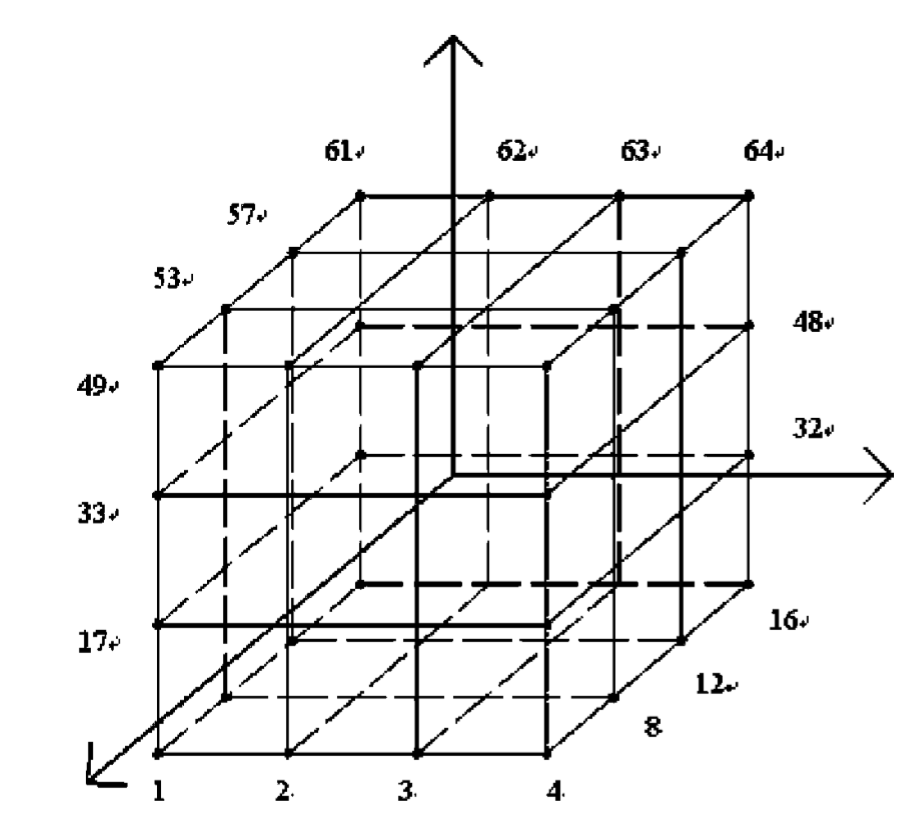
\includegraphics[width=\textwidth]{Logos/VoxelEdges.PNG}
\caption{Darstellung der lokalen 4x4x4 Nachbarschaft} 
\label{fig:nachbarschaft} 
\end{figure}
\todo{richtig bild zitieren u. evtl kleiner}




Die Funktionen für die Intensitätswerte wird im Paper mit:
\begin{equation}
	f(x,y,z) = Ax^{2}+By^{2}+Cz^{2}+2Fyz+2Gzx+2Hxy+2Ix+2Jy+2Kz+D
\end{equation}
approximiert. Da der Gradient die Ableitung der Intensitätsfunktion ist, erhält man den dreidimensionalen Gradientenvektor $n$, indem die Funktion ableitetet wird:
\begin{equation}
	n = (Ax+Gz+Hy+I, By+Fz+Hx+J, Cz + Fy + Gx + K)
\end{equation}
Um den Gradienten zu Berechnen müssen die Parameter $A,B,C,E,F,G,H,I,J,K$  berechnet werden. Dies geschieht mithilfe der Methode der kleinsten Quadrate.
\todo{methode der kleinsten quadrate genauer beschreiben}

Dies wird für jeden Voxel im Volumen berechnet. Als Ergebnis des Verfahrens kommt ein Volumen, in dem alle Gradienten gespeichert sind, heraus. Jedoch sind die Punkte um eine halbe Voxellänge verschoben. Desweiteren ist die Dimension dieses Volumens in jeder Achse um eins kleiner als das vorher gegebene Intensitätsvolumen.
Da für die Berechnung der LH-Werte jedoch der Gradient und der Intensitätswert an einer Stelle im Volumen bekannt sein muss, wurden die Intensitätswerte auf das Volumen der Gradienten umgerechnet. Dies geschieht durch eine einfach Interpolation, indem von allen 8 Nachbarn eines Punktes der Intensitätswerte aufaddiert und hinterher durch acht geteilt werden. Hierbei gehen Information verloren....
\todo{abbildung für interpolation und beschreiben was verloren geht}


Nachdem die Gradienten berechnet sind und die Intensitätswerte passend umgerechnet wurde, folgt die Berechnung der Low- und High-Werte. Dazu wird in Richtung der Gradienten integriert. Hierfür wurde wie von Nguyen auch Heun's Methode, eine modifizierte Euler Methode verwendet. Die hierzu benutzte Formel lautet:
\newline
$u_{i+1} = u_{i} + \frac{1}{2}d(\triangledown f (u_{i}) + \triangledown f(u_{i}+d \triangledown f(u_{i}))) $
\newline
Hierbei sind $u_{i}$ und $u_{i+1}$ die Positionen des aktuellen, beziehungsweise des nächsten Voxels. $\triangledown f(x)$ beschreibt den normalisierten Gradienten für die High-Werte und den normalisierten inversen Gradienten für die Low-Werte an Stelle $x$ . $d$ steht für die Schrittweite (ein Voxel).
Da das Verfahren in dieser Arbeit auf CT-Daten angewendet wird, ist das Abbruchkriterium der Integration, dass ein Gradient mit Länge null gefunden wird. Ist dies der Fall wir der Intensitätswert dieses Voxels als Ergebnis für den Low- beziehungsweise High-Wert des Startvoxel festgelegt.
\newline
Anschließend wird ein LH-Histogramm über alle berechneten Werte erstellt. Die x-Achse sind hierbei die Low- und die y-Achse die High-Werte. Deren Reichweite geht von null bis zu den jeweiligen Maxima der Werte.
\newline
Auf diesem Histogramm findet der erste Clusteringschritt  statt. Es wird ein Meanshiftclustering verwendet. Dazu wird zuerst eine Bandweite und ein Threshold gewählt, welche die Sensitivität des Clusterings bestimmen. Danach wird das Clustering für jeden Punkt im LH-Histogramm wie folgt durchgeführt.
\newline
Es werden alle Punkte die innerhalb des Radius der Bandbreite um den Startpunkt liegen gespeichert. Diese Punkte bilden nun den gefundenen Cluster. Von diesem Cluster wird der neue Mittelpunkt, der jeweilige Mittelwert der beiden Koordinaten, berechnet. Um diesen Punkt wird erneut mit selben Radius alle Punkte die bisher nicht zu dem Cluster gehören gesucht und hinzugefügt. Dies geschieht solange, bis der Abstand des neu kalkulierte Mittelpunkt zum Alten weniger als der Threshold mal die Bandweite ist. 
Nachdem das Clustering für jeden Punkt im Histogramm beendet ist, werden jene Cluster deren Mittelpunkte eine Distanz kleiner als die Hälfte der Bandweite zueinander haben miteinander zu einem einzigen Cluster verschmolzen.
\newline
\todo{intensitätswert ventrikel, vllt orginial werte nehmen und in implementierung verschiebung vorstellen}
Da die Intensitätswerte im Gehirn sehr nah beieinander liegen, wäre es nicht sinnvoll wie von Nguyen beschrieben über das komplette Histogramm mit einer Bandweite von 7\% - 9\% des maximalen LH-Wertes, das Maximum aller Low- und High-Werte, zu clustern. Das Gehirn würde dabei als ein paar wenige, sehr große Cluster erkannt werden. Diese Herangehensweise mag praktibale zum Darstellen von Knochen, des kompletter Gehirns oder anderen Bereiche sein, entspricht jedoch nicht dem Ziel dieser Arbeit, das Ventrikelsystem kenntlich zu machen und zu visualisieren. Aus diesem Grund wurde die Bandbreite des Clustering auf 0,1\% des maximalen LH-Wertes gesetzt.
\newline
Da so eine Bandbreite sehr Rechenaufwendig ist und bekannt ist, dass das Ventrikelsystem einen Intensitätswert um die ... hat, wurde desweiteren nur im Intensitätswertebereich von 1025 bis 1075 geclustert, um die Rechenzeiten gering zu halten.Weiterhin wurde nicht jeder Punkt des Histograms besucht, sondern eine Schrittweite von fünf Kasten festgelegt. Dies geschah aus der Beobachtung heraus, dass für zwei oder drei direkt nebeneinanderliegende Kasten im LH-Histogramm meist der gleiche Cluster als Ergebnis berechnet wurde. Diese wurden im letzten Schritt dann ohnehin zu einem einzigen Cluster verschmolzen, was die Berechnung jedes einzelnen Kastens unnötig machte. Diese Maßnahmen dienen ausschließlich dem Zweck Strukturen im Gehirn besser unterscheiden zu können, da sie so in verschiedene LH-Cluster eingeteilt werden und damit unterscheidbar sind. Wenn das Verfahren für andere Ziele genutzt werden soll, können die Parameter auf die von Nguyen vorgeschlagenen Werte gesetzt werden. 
\newline
Als nächstes werden die LH-Cluster erneut mit Meanshiftclustering geclustert. Diesmal jedoch anhand ihrer räumlichen Informationen im Volumen. Im Paper von Ngujen wird hierzu kein Wert für die Bandbreite vorgeschlagen. In dieser Arbeit hat sich eine Bandbreite von 10  und eine minimale Distanz vom alten zum neuen Mittelpunkt von 0,01 als zielführend erwiesen.
\newline
Nachdem alle Cluster erzeugt wurden, werden ihnen zufällige IDs von eins bis zur Anzahl an Clustern zugeteilt. Anschließend wird ein Volumen erstellt, mit den Dimensionen des ursprünglichen Intensitätsvolumens, dass nur mit nullen als Werte gefüllt ist. Warum es diese Dimension haben muss, wird später erklärt. Danach wird durch alle Cluster iteriert, und jeder Voxel in das neu erstellte Volumen an der jeweiligen Position eingetragen. Dabei ist der eingetragene Wert immer die  ID des aktuellen Clusters. Nachdem alle Cluster abgearbeitet wurden, besteht das Volumen aus ausschließlich nullen und den IDs der Cluster an den passenden Stellen.
\newline
Dieses Volumen wird als eine binäre Datei abgespeichert und in Unity geladen. Hier kann der Anwender sich entweder die Form von einzelnen IDs anschauen oder eine Reichweite von IDs. Die gewählten IDs werden rot markiert und sich deutlich vom restlichen Volumen zu unterscheiden. Mithilfe der Darstellung muss der Nutzer anhand der Form die Cluster erkennen, die zum Ventrikelsystem gehören, und deren IDs notieren. 
\newline
Hat er dies getan kann er im ... Programm die binäre Datei mit den IDs, die ursprüngliche Intensitätsvolumendatei laden und eine die Liste der passenden IDs als Parameter übergeben. Die ausgewählten IDs werden zu einem Cluster verschmolzen und in das Intensitätsvolumen übernommen. Dort erhalten sie, da der maximale Wert von CT-Daten bei ...(4400) liegt, den Wert 5000. Dieser Wert erhöht das Maximum für die Darstellung der Daten nur gering, ist dafür aber im Volumen sonst nirgends enthalten. Das Ergebnis dieser Verschmelzung wird wieder als binäre Datei gespeichert.
\newline
Als letzten Schritt kann nun der Benutzer die verschmolzene Datei erneut in Unity laden. Hier kann er sich dann das Volumen normale abhängig von den Grauwerten dargestellt anzeigen lassen, mit dem Ventrikelsystem in rot, oder einer anderen ausgewählten Farbe darin.
\newline
\todo{letzten schritt genauer}

